\documentclass[openany, a4paper,12pt]{book}

\usepackage{amsmath,amssymb,amsthm, amsfonts,mathrsfs}
\usepackage{geometry}
\usepackage{enumerate}
\usepackage{pdfpages}
\usepackage{subcaption}
\usepackage{graphicx}
\usepackage{cite}
\usepackage{tikz-cd} %交换图
\usepackage{tikz}


\usepackage{stix} %symbols and text fonts
\usepackage{charter}
\usepackage[T1]{fontenc}

\usepackage{xcolor}                             % Link color
 \definecolor{custom-blue}{RGB}{0,99,166} 
\usepackage{hyperref}
\hypersetup{
    colorlinks=true, % 启用彩色链接
    linkcolor=purple,  % 普通内部链接的颜色
    citecolor=blue,  % 引用链接的颜色
    filecolor=green,  % 打开本地文件的链接颜色
    urlcolor=red    % 链接到URL的颜色
}

\usepackage{titlesec}  % 用于修改章节标题的格式

% 使用 \titleformat 定义新的 \section 和 \subsection 样式
\titleformat{\section}[block]
  {\normalfont\Large\bfseries}    % 标题字体样式
  {\S\ \thesection}               % 在标题前加上 \S 和节编号
  {1em}                           % 标题和编号之间的间距
  {}                               % 标题后面的内容

\titleformat{\subsection}[block]
  {\normalfont\large\bfseries}    % 子节标题字体样式
  {\S\ \thesubsection}            % 在子节标题前加上 \S 和子节编号
  {1em}                           % 标题和编号之间的间距
  {}                               % 标题后面的内容

  \titleformat{\chapter}[block]
  {\centering\Huge\bfseries}    
  {Chapter \thechapter }           % 居中
  {1em}                           
  {} 

%%%%%%%%页面与页面对齐
\textwidth=6.5in
\textheight=8.7in
\topmargin=0in
\oddsidemargin=0in
\evensidemargin=0in



%%Bold the titles
\makeatletter
\def\th@plain{%
  \thm@notefont{}% same as heading font
  \itshape % body font
}
\def\th@definition{%
  \thm@notefont{}% same as heading font
  \normalfont % body font
}
\makeatother

\newtheorem{theorem}{Theorem}[section]
\newtheorem*{theorem*}{Theorem}
\newtheorem{lemma}[theorem]{Lemma}
\newtheorem{corollary}[theorem]{Corollary}
\newtheorem{proposition}[theorem]{Proposition}
\newtheorem{conjecture}[theorem]{Conjecture}

\theoremstyle{definition}
\newtheorem{definition}[theorem]{Definition}
\newtheorem{example}[theorem]{Example}
\newtheorem{exercise}[theorem]{Exercise}
\newtheorem{problem}[theorem]{Problem}
\newtheorem{remark}{Remark}[section]
\newtheorem{question}{Question}[section]
\renewcommand*{\thequestion}{\Alph{question}}

\DeclareMathOperator{\grad}{grad}
\DeclareMathOperator{\dimension}{dim}
\DeclareMathOperator{\trace}{tr} 
\DeclareMathOperator{\di}{div}
\DeclareMathOperator{\ricci}{Ricci}
\DeclareMathOperator{\dist}{dist}
\DeclareMathOperator{\hess}{Hess}


\DeclareMathOperator{\im}{Im}

\def\zz{{\mathbb Z}}
\def\rr{{\mathbb R}}
\def\cc{{\mathbb C}}
\def\qq{{\mathbb Q}}
\def\nn{{\mathbb N}}
\def\ss{{\mathbb S}}
\def\oo{{\infty}}

\newcommand{\la}{\langle}
\newcommand{\ra}{\rangle}

\newcommand{\dif}{\mathop{}\!\mathrm{d}} % unicode-math 

\newtheoremstyle{coloredtheorem4}
  {\topsep}   
  {\topsep}   
{\normalfont} 
  {}          
  {\color{gray}\bfseries}
  {.}        
  {.5em}      
  {\thmname{#1}\thmnumber{ #2}\thmnote{ (#3)}} 



%%% 标题有数学符号, 请使用: \texorpdfstring{$\phi$}{name}

\def\crm{{(M,T_{1,0}(M))}}

\usetikzlibrary{positioning, fit, calc}   
\tikzset{block/.style={draw, thick, text width=2cm ,minimum height=1.3cm, align=center},   
line/.style={-latex}     
}  

\begin{document}

\title{CR Geometry}
\author{L}
\date{2025 Spring}
\maketitle



% 前置部分包含目录、中英文摘要以及符号表等
% \frontmatter

% 目录
\tableofcontents

\chapter{Symplectic Manifolds}

\section{Symplectic Manifolds}

\begin{definition}
    By a \textbf{symplectic manifold} we mean an even-dimensional differentiable $\left(C^{\infty}\right)$ manifold $M^{2 n}$ together with a global 2-form $\Omega$ which is closed and of maximal rank, i.e., $d \Omega=0, \Omega^n \neq 0$. 
    
    By a \textbf{symplectomorphism} $f:\left(M_1, \Omega_1\right) \longrightarrow\left(M_2, \Omega_2\right)$ we mean a diffeomorphism $f: M_1 \longrightarrow M_2$ such that 
    $$f^* \Omega_2=\Omega_1.$$
\end{definition}

\begin{definition}
    Let $\iota: L \longrightarrow M^{2 n}$ be an immersion into a symplectic manifold $\left(M^{2 n}, \Omega\right)$. We say that $L$ is a \textbf{Lagrangian submanifold} if the dimension of $L$ is $n$ and $\iota^* \Omega=0$.
\end{definition}

\begin{theorem}[Weistein]
    If $L$ is a Lagrangian submanifold of a symplectic manifold $(M, \Omega)$, then there exists a neighborhood of $L$ in $M$ that is symplectomorphic to a neighborhood of the zero section in $T^{*}L$.
\end{theorem}

\begin{theorem}
    Let $X$ be a symplectic vector field on $(M, \Omega), g$ an associated metric, and $J$ the corresponding almost complex structure. Then $X^i=J^{i k} \theta_k$ for some closed 1-form $\theta$. Conversely, given a closed 1-form $\theta, X^i=J^{i k} \theta_k$ defines a symplectic vector field.
\end{theorem}
\begin{corollary}
    For $f \in C^{\infty}(M), J \nabla f$ is symplectic, where $\nabla f$ is the gradient of $f$. Conversely, given $X$ symplectic, $X$ is locally $J \nabla f$.
\end{corollary}


\begin{theorem}[Hatakeyama, 1966]
    The group of symplectomorphisms acts transitively on a compact symplectic manifold $(M, \Omega)$.
\end{theorem}


\subsection{Examples}
\begin{example}
    Let $M$ be a differentiable manifold. Then its cotangent bundle $T^* M$ has a natural symplectic structure. For $z \in T^* M$ and $V$ in the tangent space of $T^* M$ at $z, T_z T^* M$, define a 1 -form $\beta$, often called the \textbf{Liouville form}, by $\beta(V)_z=z\left(\pi_* V\right)$, where $\pi: T^* M \longrightarrow M$ is the projection map. If $x^1, \ldots, x^n$ are local coordinates on $M$, then $q^i=x^i \circ \pi$ together with fiber coordinates $p^1, \ldots, p^n$ give local coordinates on $T^* M$. In these coordinates $\beta$ has the local expression $\sum_{i=1}^n p^i d q^i$. The natural symplectic structure on $T^* M$ is given by $\Omega=-d \beta$.
\end{example}



\section{Contact manifolds}
\begin{definition}
    By a \textbf{contact manifold} we mean a $C^{\infty}$ manifold $M^{2 n+1}$ together with a 1 -form $\eta$ such that 
    \begin{equation}
        \eta \wedge(d \eta)^n \neq 0. 
    \end{equation}
\end{definition}
\begin{remark}
   1)  In particular, $\eta \wedge(d \eta)^n \neq 0$ is a volume element on $M$, so that a contact manifold is orientable. 
    
   2) we have a global vector field $\xi$ satisfying
    \begin{equation}
        d \eta(\xi, X)=0, \quad \eta(\xi)=1 .
    \end{equation}
$\xi$ is called the \textbf{characteristic vector field} or \textbf{Reeb vector field } of the contact structure $\eta$. 

3) By formula $\left.\left.L_{\xi}=d \circ(\xi\lrcorner\right)+(\xi\lrcorner\right) \circ d$, we have immediately that
\begin{equation}
    L_{\xi} \eta=0, \quad L_{\xi} d \eta=0 .
\end{equation}
\end{remark}

\begin{definition}
    We denote by $\mathcal{D}$ the \textbf{contact distribution} or subbundle defined by the subspaces $\mathcal{D}_m=\left\{X \in T_m M: \eta(X)=0\right\}$. 
\end{definition}
\begin{remark}
    Roughly speaking, the meaning of the contact condition, $\eta \wedge(d \eta)^n \neq 0$, is that the contact subbundle is as far from being integrable as possible; in particular, $\mathcal{D}$ rotates as one moves around on the manifold. For a subbundle defined by a 1 -form $\eta$ to be integrable it is necessary and sufficient that 
    \begin{equation}
        \eta \wedge(d \eta) \equiv 0. 
    \end{equation}
\end{remark}

\begin{definition}
    A contact structure is \textbf{regular} if $\xi$ is \textbf{regular} as a vector field, that is, every point of the manifold has a neighborhood such that any integral curve of the vector field passing through the neighborhood passes through only once. 
\end{definition}
\begin{remark}
    Two well-known examples of nonregular vector fields on surfaces are the irrational flow on a torus and the flow around a Möbius band.
\end{remark}

\begin{theorem}[\textbf{Darboux coordinate system}]
    About each point of a contact manifold $\left(M^{2 n+1}, \eta\right)$ there exist local coordinates $\left(x^1, \ldots, x^n, y^1, \ldots, y^n, z\right)$ with respect to which
    \begin{equation}
        \eta=d z-\sum_{i=1}^n y^i d x^i.
    \end{equation}
\end{theorem}
\begin{remark}
    There are many similar results in this spirit.
\end{remark}

\begin{definition}
    A diffeomorphism $f$ of $M^{2 n+1}$ or between open subsets of $\mathbb{R}^{2 n+1}$ with the contact structure of the Darboux form of the above theorem is called a \textbf{contact transformation} if 
    \begin{equation}
        f^* \eta=\tau \eta
    \end{equation}
    for some nonvanishing function $\tau$ on the domain of $f$. If $\tau \equiv 1, f$ is called a \textbf{strict contact transformation}.
\end{definition}

\begin{definition}
    There is also the notion of a \textbf{contact structure in the wider sense,} often called simply a "contact structure" by many authors, which can be defined in a number of ways. For example, a contact manifold in the wider sense is a manifold with a differentiable structure modeled on the pseudogroup of contact transformations on $\mathbb{R}^{2 n+1}$.
\end{definition}

\begin{theorem}
 Let $M^{2 n+1}$ be a contact manifold in the wider sense. If $n$ is odd, then $M^{2 n+1}$ is orientable.
\end{theorem}
\begin{theorem}
     Let $M^{2 n+1}$ be a contact manifold in the wider sense. If $n$ is even and $M^{2 n+1}$ is orientable, then $M^{2 n+1}$ is a contact manifold.
\end{theorem}

\begin{theorem}
    Let $M^{2 n+1}$be a contact manifold in the wider sense which is not a contact manifold in the restricted sense. Then its 2-fold covering manifold is a contact manifold in the restricted sense.
\end{theorem}

\begin{theorem}[\textbf{Boothby-Wang fibration}]
     Let $\left(M^{2 n+1}, \eta^{\prime}\right)$ be a compact regular contact manifold. Then there exists a contact form $\eta=\tau \eta^{\prime}$ for some nonvanishing function $\tau$ whose characteristic vector field $\xi$ generates a free effective $S^1$ action on $M^{2 n+1}$. Moreover, $M^{2 n+1}$ is the bundle space of a principal circle bundle $\pi: M^{2 n+1} \longrightarrow M^{2 n}$ over a symplectic manifold $M^{2 n}$ whose symplectic form $\Omega$ determines an integral cocycle on $M^{2 n}$ and $\eta$ is a connection form on the bundle with curvature form $d \eta=\pi^* \Omega$.
\end{theorem}

\begin{definition}[Other notions]
    \textbf{periodic point, planar, almost regular/quasi-regular, R-contact manifold}, etc..
\end{definition}

\subsection{Examples}
\begin{example}
    The cotangent sphere bundle and the tangent sphere bundle of a Riemannian manifold are contact manifolds.
\end{example}

\begin{example}
    Let $M$ be an $n$-dimensional manifold and $T^* M$ its cotangent bundle. As in the previous example we can define a 1 -form $\beta$ by the local expression $\beta=\sum_{i=1}^n p^i d q^i$. Let $M^{2 n+1}=T^* M \times \mathbb{R}, t$ the coordinate on $\mathbb{R}$, and $\mu: M^{2 n+1} \longrightarrow T^* M$ the projection to the first factor. Then $\eta=d t-\mu^* \beta$ is a contact form on $M^{2 n+1}$.
\end{example}

\section{Associated Metrics}
\begin{definition}
    An \textbf{almost complex structure} is a tensor field $J$ of type $(1,1)$ such that $J^2=-I$. A \textbf{Hermitian metric} on an almost complex manifold $(M, J)$ is a Riemannian metric that is invariant by $J$, i.e.,
    \begin{equation}
        g(J X, J Y)=g(X, Y).
    \end{equation}
    \end{definition}

    \begin{remark}
        Note also that every almost complex manifold admits a Hermitian metric, for if $k$ is any Riemannian metric, then $g$ defined by
        \begin{equation}
            g(X, Y)=k(X, Y)+k(J X, J Y)
        \end{equation}
is Hermitian.
    \end{remark}
    
    \begin{definition}
    Noting that $J$ is negative self-adjoint with respect to $g$, i.e., $g(X, J Y)=$ $-g(J X, Y)$, therefore 
    \begin{equation}
         \Omega(X, Y)=g(X, J Y)
    \end{equation}
    defines a 2 -form called the\textbf{ fundamental 2-form} of the \textbf{almost Hermitian structure} $(M, J, g)$. If 
    \begin{equation}
            d \Omega= 0,
    \end{equation}
 the structure is \textbf{almost Kähler}. If $M$ is a complex manifold and $J$ the corresponding almost complex structure, we say that $(M, J, g)$ is a \textbf{Hermitian manifold}.
\end{definition}
\begin{definition}
    Given $(M, J, g)$ we can construct a particular local orthonormal basis as follows. Let $\mathcal{U}$ be a coordinate neighborhood on $M$ and $X_1$ any unit vector field on $\mathcal{U}$. Let $X_{1^*}=J X_1$. Now choose a unit vector field $X_2$ orthogonal to both $X_1$ and $X_{1^*}$. Then $J X_2$ is also orthogonal to $X_1$ and $X_{1^*}$. Continuing in this manner we have a local orthonormal basis of the form $\left\{X_1, \ldots, X_n, J X_1, \ldots, J X_n\right\}$. Such a basis is called a \textbf{$J$-basis.} 
\end{definition}

\begin{remark}
    An almost complex (almost Hermitian) structure on $M$ can be thought of as a reduction of the structural group to $U (n)$.
\end{remark}

\begin{remark}
    The structural group of a symplectic manifold is reducible to $U(n)$ and that of a contact manifold to $U(n) \times 1$ (Chern [1953]). 
\end{remark}
\begin{definition}
        For an odd-dimensional manifold $M^{2 n+1}$, J. Gray [1959] defined \textbf{an almost contact structure} as a reduction of the structural group to $U(n) \times 1$. In terms of structure tensors we say that $M^{2 n+1}$ has an almost contact structure or sometimes \textbf{$(\phi, \xi, \eta)$-structure} if it admits a tensor field $\phi$ of type $(1,1)$, a vector field $\xi$, and a 1 -form $\eta$ satisfying
    \begin{equation}
        \phi^2=-I+\eta \otimes \xi, \quad \eta(\xi)=1 .
    \end{equation}
\end{definition}
\begin{theorem}
    Suppose $M^{2 n+1}$ has a $(\phi, \xi, \eta)$-structure. Then 
    \begin{equation}
        \phi \xi=0, \quad \eta \circ \phi=0.
    \end{equation}
 Moreover, the endomorphism $\phi$ has rank $2 n$.
\end{theorem}

\begin{definition}
    If a manifold $M^{2 n+1}$ with a $(\phi, \xi, \eta)$-structure admits a Riemannian metric $g$ such that
    \begin{equation}\label{eq12}
        g(\phi X, \phi Y)=g(X, Y)-\eta(X) \eta(Y),
    \end{equation}
we say that $M^{2 n+1}$ has an \textbf{almost contact metric structure} and $g$ is called a \textbf{compatible metric}. 
\end{definition}
\begin{remark}
    For any $X\in \mathcal{D}$, let $Y=\xi$ in $\eqref{eq12}$, we get 
    $g(\phi(X),\xi)=0$, thus
    \begin{equation}
        \phi (\mathcal{D}) \subset \mathcal{D}.
    \end{equation}
\end{remark}

\begin{remark}
        As in the almost Hermitian case, we define a 2 -form, called the fundamental 2-form of the almost contact metric structure, by 
        \begin{equation}
            \Phi(X, Y)=g(X, \phi Y). 
        \end{equation}
\end{remark}
\begin{remark}
    Also as in the case of an almost complex structure, the existence of the compatible metric is easy. For if $k^{\prime}$ is any metric, first set $k(X, Y)=k^{\prime}\left(\phi^2 X, \phi^2 Y\right)+\eta(X) \eta(Y)$; then $\eta(X)=k(X, \xi)$. Now define $g$ by
    \begin{equation}
        g(X, Y)=\frac{1}{2}(k(X, Y)+k(\phi X, \phi Y)+\eta(X) \eta(Y)).
    \end{equation}
\end{remark}


\begin{remark}
    Setting $Y=\xi$ we have immediately that
\begin{equation}
    \eta(X)=g(X, \xi).
\end{equation}
\end{remark}
\begin{remark}
    We can obtain a local orthonormal basis $\left\{X_i, X_{i^*}=\phi X_i, \xi\right\}$, called a \textbf{$\phi$-basis}.
\end{remark}
\begin{remark}
    Given a manifold $M^{2 n+1}$ with a $(\phi, \xi, \eta)$-structure, let $g$ be a compatible metric, then proceeding as in the almost complex case, we see that the structural group of $M^{2 n+1}$ is reducible to $U(n) \times 1$. 
\end{remark}

\begin{theorem}[\textbf{Existence of associated metrics 1}]
    Let $\left(M^{2 n}, \Omega\right)$ be a symplectic manifold. Then there exist a Riemannian metric $g$ and an almost complex structure $J$ such that
$$
g(X, J Y)=\Omega(X, Y) .
$$
\end{theorem}

\begin{definition}
    In particular, given a symplectic manifold $\left(M^{2 n}, \Omega\right)$, we say that a Riemannian metric $g$ is an \textbf{associated metric} if there exists an almost complex structure $J$ such that 
    $$g(X, J Y)=\Omega(X, Y).$$
\end{definition}

\begin{theorem}[\textbf{Existence of associated metrics 2}]
    Let $\left(M^{2 n+1}, \eta\right)$ be a contact manifold and $\xi$ its characteristic vector field. Then there exists an almost contact metric structure such that 
    $$g(X, \phi Y)=d \eta(X, Y).$$
\end{theorem}

\begin{definition}
    As in the symplectic case, given a contact manifold $\left(M^{2 n+1}, \eta\right)$, we say that a Riemannian metric $g$ is an \textbf{associated metric} if there exists an almost contact metric structure such that 
   $$g(X, \phi Y)=d \eta(X, Y).$$
    In this case we also speak of a\textbf{ contact metric structure}; other authors often use the phrase contact Riemannian structure. 
\end{definition}
\begin{definition}[Alternative definition]
    Working strictly with structure tensors, one may avoid the polarization process by defining an associated metric as follows: Given a contact manifold $\left(M^{2 n+1}, \eta\right)$ with characteristic vector field $\xi$, a Riemannian metric $g$ is an associated metric if, first of all,
$$
\eta(X)=g(X, \xi)
$$
and secondly, there exists a tensor field $\phi$ of type $(1,1)$ such that
$$
\phi^2=-I+\eta \otimes \xi, \quad d \eta(X, Y)=g(X, \phi Y) .
$$
\end{definition}
\begin{proof}
    Only need to verify 
    \begin{equation}
        g(X,\phi Y)+g(\phi  X,Y)=0, X,Y \in \mathcal{D}.
    \end{equation}
    But it follows immediately by symmetry of $g$ and antisymmetry of $d\eta$.
\end{proof}
\begin{remark}
    Caution that it is possible to have a contact manifold $\left(M^{2 n+1}, \eta\right)$ with characteristic vector field $\xi$ and an almost contact metric structure $(\phi, \xi, \eta, g)$, same $\xi$ and $\eta$, without $g(X, \phi Y)=d \eta(X, Y)$.
\end{remark}
\begin{remark}
    On the other hand, it is possible for a Riemannian metric g to be an associated metric for more than one symplectic structure. For example, on a hyper-Kähler manifold one has, by definition, three independent global Kähler structures $\left(J_a, g\right), a=1,2,3$, satisfying $J_1 J_2+J_2 J_1=0$, $J_3=J_1 J_2$. Thus the three fundamental 2 -forms give three symplectic structures with $g$ an associated metric for each of them.
\end{remark}

\begin{theorem}
     On a contact metric manifold the integral curves of $\xi$ are geodesics.
\end{theorem}
\begin{proof}
    For a contact metric structure we have
$$
0=\left(L_{\xi} \eta\right)(X)=\xi g(X, \xi)-g\left(\nabla_{\xi} X-\nabla_X \xi, \xi\right)=g\left(X, \nabla_{\xi} \xi\right),
$$
so the integral curves of $\xi$ are geodesics.
\end{proof}


\begin{remark}
    The set $\mathcal{A}$ of all associated metrics forms a infinite-dimensional sapce.
\end{remark}

\begin{theorem}
     Let $\left(M^{2 n}, \Omega\right)$ be a symplectic manifold (resp. $\left(M^{2 n+1}, \eta\right)$ a contact manifold) and $g$ an associated metric. Then
     \begin{equation}
     d V=\frac{(-1)^n}{2^n n !} \Omega^n\left(\text { resp. } d V=\frac{(-1)^n}{2^n n !} \eta \wedge(d \eta)^n\right).
     \end{equation}
\end{theorem}
\begin{remark}
    Not sure if it's correct up to some factors.
\end{remark}

\begin{definition}
    $\mathcal{A}$: the set of all associated metrics
    
    $\mathcal{N}$: the set of all metrics with the same volume element
    
    $\mathcal{M}$: the set of all metrics
\end{definition}
\begin{definition}
    For symmetric tensor fields $S$ and $T$ of type $(0,2)$ we define a Riemannian metric $(\cdot, \cdot)$ by
    \begin{equation}
        (S, T)_g=\int_M S_{i j} T_{k l} g^{i k} g^{j l} d V_g.
    \end{equation}
\end{definition}
\begin{remark}
    One can think of metrics with the same total volume on an n-dimensional manifold as being at a fixed distance from the zero tensor.
\end{remark}
\begin{proof}
    Consider the path $t g, t \in[0,1]$, from the zero tensor to the metric $g$; then since $g$ may be considered as the tangent to the path at each point, we have the following entertaining computation:
$$
|g| \equiv \int_0^1(g, g)_{t g}^{1 / 2} d t=\int_0^1\left(\frac{n}{t^2} \int_M \sqrt{t^n \operatorname{det} g} d x^1 \cdots d x^n\right)^{1 / 2} d t=4 \sqrt{\frac{\operatorname{vol}_g M}{n}}.
$$
\end{proof}


\begin{proposition}
    On a compact manifold $M$ the set $\mathcal{M}$ of all Riemannian metrics may be given a Riemannian metric (Ebin [1970]): The tangent space, $T_g \mathcal{M}$, of $\mathcal{M}$ at a metric $g$ is the space of symmetric tensor fields of type $(0,2)$.

    The tangent space $T_g\mathcal{A}$ of $\mathcal{A}$ at $g$ is the set of all symmetric tensor fields that anticommute with $J$ ($\phi$ and annihilate $\xi$).
\end{proposition}

\begin{theorem}
    Let $(M, \Omega)$ be a symplectic manifold, or respectively $(M, \eta)$ a contact manifold, and $f$ a diffeomorphism satisfying $f^* \Omega=\Omega$, respectively $f^* \eta=\eta$. Then for any associated metric $g, f^* g$ is also an associated metric.
\end{theorem}

\begin{lemma}
    Let $(M, g)$ be a compact orientable Riemannian manifold and for a vector field $V$ let $v(X)=g(V, X)$. Then $\int_M V^i \theta_i d V_g=0$ for every closed 1-form $\theta$ if and only if $v=\delta \Psi$ for some 2 -form $\Psi$. $\int_M v_i X^i d V_g=0$ for every vector field $X$ if and only if $v=0$.
\end{lemma}

\section{Examples of almost contact metric manifolds}

\begin{example}
    $\mathbb{R}^{2n+1}(-3).$ It's a contact metric structure on it.
\end{example}

\begin{example}
    $M^{2n+1}\subset \tilde{M}^{2n+2}$. Every $C^{\infty}$ orientable hypersurface of an almost complex manifold has an almost contact structure.

    In general, one cannot expect the induced almost contact metric structure to be a contact metric structure.
\end{example}
\begin{theorem}
    Let $M^{2 n+1}$ be a hypersurface of a Kähler manifold $\tilde{M}^{2 n+2},(\phi, \xi, \eta, g)$ its induced almost contact metric structure and $A$ its Weingarten map. Then $(\phi, \xi, \eta, g)$ is a contact metric structure if and only if 
    \begin{equation}
        A \phi+\phi A=-2 \phi.
    \end{equation}
\end{theorem}

\begin{example}
    $S^5\subset S^6$.
\end{example}

\begin{example}[The Boothby–Wang fibration]
   It has a \textbf{$K$-contact structure}.
\end{example}

\begin{definition}
    A contact metric structure for which the characteristic vector field is a Killing vector field is called a \textbf{$K$-contact structure}.
\end{definition}

\begin{theorem}
    Let $\pi: M^{2n+1}\to M^{2n}$ be the Boothby-Wang fibration of a compact regular contact manifold $M^{2n+1}$. Then the first Betti numbers of  $M^{2n+1}$ and $M^{2n}$ are equal.
\end{theorem}
\begin{theorem}
    No torus $T^{2n+1}$ can carry a regular contact structure.
\end{theorem}

\begin{example}
    $M^{2n}\times \mathbb{R}$. It is an almost contact metric structure that is certainly not a contact metric structure.
\end{example}

\begin{example}[Parallelizable manifolds]
In particular, any odd-dimensional Lie group carries an almost contact structure.
\end{example}
\begin{definition}
    A smooth manifold with or without boundary is said to be \textbf{parallelizable} if it admits a smooth global frame.
\end{definition}
\begin{theorem}
    A smooth vector bundle is smoothly trivial if and only if it admits a smooth global frame.
\end{theorem}


\section{Integral Submanifolds and Contact Transformations}

\subsection{Integral submanifolds}
Let $M^{2 n+1}$ be a contact manifold with contact form $\eta$. We have seen that $\eta=0$ defines a $2 n$-dimensional subbundle $\mathcal{D}$ called the \textbf{contact distribution} or\textbf{ subbundle} and that since $\eta \wedge(d \eta)^n \neq 0, \mathcal{D}$ is nonintegrable.

\begin{definition}
    A submanifold $M^r$ of $M^{2 n+1}$ is called an \textbf{integral submanifold} if $\eta(X)=0$ for every tangent vector $X$. It is clear that for any pair of tangent vector fields we have
$$
d \eta(X, Y)=\frac{1}{2}(X \eta(Y)-Y \eta(X)-\eta([X, Y])=0 .
$$

Then in terms of associated metrics, $g(X, \phi Y)=0$ and for this reason integral submanifolds are often called $C$-\textbf{totally real submanifolds.} In particular, $\phi$ maps tangent vectors to normal vectors; also, since $\xi$ is a normal vector, the dimension $r$ can be at most $n$. On the other hand, by the Darboux theorem, it's easy to see there exist an $n$-dim integral submanifold.
\end{definition}

\begin{theorem}
    Let $M^{2n+1}$ be a contact manifold with contact form $\eta$. Then there exist integral submanifolds of the contact subbundle $\mathcal{D}$ of dimension $n$ but of no higher dimension.
\end{theorem}

\begin{theorem}[Sasaki, 1964]
     Let $\left(x^i, y^i, z\right), i=1, \ldots, n$, be local coordinates about a point $m=\left(x_0^i,  y_0^i, z_0\right)$ such that $\eta=d z-\sum_{i=1}^n y^i d x^i$ on the coordinate neighborhood. In order that $r$ linearly independent vectors $X_\lambda, \lambda=$ $1, \ldots, r \leq n$, at $m$ with components $\left(a_\lambda^i, b_\lambda^i, c_\lambda\right)$ be tangent to an $r$ dimensional integral submanifold it is necessary and sufficient that $\eta\left(X_\lambda\right)=0$ and $d \eta\left(X_\lambda, Y_\mu\right)=0$, that is, $c_\lambda=\sum_i y_0^i a_\lambda^i$ and $\sum_i a_\lambda^i b_\mu^i=$ $\sum_i a_\mu^i b_\lambda^i$.
\end{theorem}

As in the symplectic case we note the abundance of integral submanifolds of $\mathcal{D}$.

\begin{theorem}[Sasaki, 1964]
    Given a vector $X \in \mathcal{D}$ at $m \in M^{2n+1}$ and any $r, 1 \leq r \leq n$, there exists an $r$-dimensional integral submanifold $M^r$ of $\mathcal{D}$ through m with $X$ tangent to $M^r$.
\end{theorem}

Similar to Weistein theorem, we have 
\begin{theorem}[Lychagin, 1977]
     If $L$ is an n-dimensional integral submanifold of a contact manifold $\left(M^{2 n+1}, \eta\right)$, then there exist an open neighborhood $\mathcal{U}$ of $L$ in $M^{2 n+1}$, an open neighborhood $\mathcal{V}$ of the zero section in $T^* L \times \mathbb{R}$, and a diffeomorphism $f: \mathcal{U} \longrightarrow \mathcal{V}$ such that $\left.f\right|_L$ is the identity on $L$ and $f^*(\beta-d t)=\eta$.
\end{theorem}

\subsection{Contact transformations}
Recall that a diffeomorphism $f$ of $M^{2 n+1}$ is a contact transformation if $f^* \eta=\tau \eta$ for some nonvanishing function $\tau$ and that $f$ is a strict contact transformation if $\tau \equiv 1$. Clearly $f^* d \eta=d \tau \wedge \eta+\tau d \eta$, so if $d \eta$ is invariant, $(\tau-1) d \eta=-d \tau \wedge \eta$ and hence $(\tau-1) \eta \wedge d \eta=0$, giving $\tau \equiv 1$. Thus $f$ is strict if and only if $d \eta$ is invariant.

\begin{theorem}
    $f$ is a contact transformation if and only if $X \in \mathcal{D}$ implies $f_* X \in \mathcal{D}$.
\end{theorem}

\begin{theorem}
    A diffeomorphism $f$ is a contact transformation if and only if $f$ maps $r$-dimensional integral submanifolds to $r$-dimensional integral submanifolds.
\end{theorem}

\begin{definition}
    If $L_{X}\eta=\sigma \eta$ for some function $\sigma$, $X$ is called an \textbf{infinitesimal contact transformation}.If $\sigma=0$,  we say that $X$ is a \textbf{strict infinitesimal contact transformation}.
\end{definition}

\begin{theorem}
    A vector field $X$ is an infinitesimal contact transformation if and only if there exists a function $f$ on $M^{2n+1}$ such that 
    \begin{equation}
        X = -\frac{1}{2} \phi \nabla f + f\xi.
    \end{equation}
\end{theorem}
\begin{proof}
    For sufficiency, we have 
    \begin{equation}
        L_{X}\eta=(\xi f) \eta.
    \end{equation}
    ...
\end{proof}

\begin{corollary}
    $X$ is strict if and only if $\xi f=0.$
\end{corollary}

As in the symplectic case we have the following theorem of Hatakeyama on the transitivity of the group of contact transformations.
\begin{theorem}[Hatakeyama, 1966]
    Let $ M^{2n+1}$ be a compact contact manifold. Then for any two points $p, q$, there exists a contact transformation mapping $p$ to $q$. If $M^{2n+1}$ is regular, there exists a strict contact transformation mapping $p$ to $q$.
\end{theorem}


\section{Sasakian and Cosymplectic Manifolds}

Let $M^{2 n+1}$ be an almost contact manifold with structure tensors $(\phi, \xi, \eta)$ and consider the manifold $M^{2 n+1} \times \mathbb{R}$. We denote a vector field on $M^{2 n+1} \times \mathbb{R}$ by $(X, f \frac{d}{d t})$, where $X$ is tangent to $M^{2 n+1}, t$ the coordinate on $\mathbb{R}$, and $f$ a $C^{\infty}$ function on $M^{2 n+1} \times \mathbb{R}$. Define an almost complex structure $J$ on $M^{2 n+1} \times \mathbb{R}$ by
$$
J\left(X, f \frac{d}{d t}\right)=\left(\phi X-f \xi, \eta(X) \frac{d}{d t}\right)
$$
that $J^2=-I$ is easy to check. If now $J$ is integrable, we say that the almost contact structure $(\phi, \xi, \eta)$ is \textbf{normal} (Sasaki and Hatakeyama [1961]).

\begin{remark}
    Compare to the ``regular''.
\end{remark}

\begin{definition}
    We are thus led to define four tensors $N^{(1)}, N^{(2)}, N^{(3)}, N^{(4)}$ by
    \begin{equation}
        \begin{aligned}
N^{(1)}(X, Y) & =[\phi, \phi](X, Y)+2 d \eta(X, Y) \xi, \\
N^{(2)}(X, Y) & =\left(L_{\phi X} \eta\right)(Y)-\left(L_{\phi Y} \eta\right)(X), \\
N^{(3)} & =\left(L_{\xi} \phi\right) X \\
N^{(4)} & =\left(L_{\xi} \eta\right)(X) .
\end{aligned}
    \end{equation}
\end{definition}

\begin{theorem}
    For an almost contact structure $(\phi, \xi, \eta)$ the vanishing of $N^{(1)}$ implies the vanishing of $N^{(2)}, N^{(3)}$ and $N^{(4)}$.
\end{theorem}
\begin{theorem}
     For a contact structure $(\phi, \xi, \eta, g)$, $N^{(2)}$ and $N^{(4)}$ vanish. Moreover, $N^{(3)}$ vanishes if and only if $\xi$ is a Killing vector field.
\end{theorem}

\begin{lemma}
     For an almost contact metric structure $(\phi, \xi, \eta, g)$, the covariant derivative of $\phi$ is given by
     \begin{equation}
         \begin{aligned}
2 g\left(\left(\nabla_X \phi\right) Y, Z\right)= & 3 d \Phi(X, \phi Y, \phi Z)-3 d \Phi(X, Y, Z)+g\left(N^{(1)}(Y, Z), \phi X\right) \\
& +N^{(2)}(Y, Z) \eta(X)+2 d \eta(\phi Y, X) \eta(Z) \\
& -2 d \eta(\phi Z, X) \eta(Y).
\end{aligned}
     \end{equation}
\end{lemma}

\begin{definition}
Define  a tensor
    \begin{equation}
        h:=\frac{1}{2}\left(L_{\xi} \phi\right) X=\frac{1}{2}N^{(3)}.
    \end{equation}
\end{definition}
\begin{remark}
    The first property to note is immediate, namely $h \xi=0$. 
\end{remark}

\begin{lemma}
    On a contact metric manifold $h$ is a symmetric operator,
    \begin{equation}
        \nabla_X \xi=-\phi X-\phi h X.
    \end{equation}
$h$ anticommutes with $\phi$, and $\operatorname{tr} h=0$.
\end{lemma}
\begin{corollary}
    On a contact metric manifold $\delta \eta=0$.
\end{corollary}

\subsection{Definition of Sasakian manifolds}

\begin{definition}
    A Sasakian manifold is a normal contact metric manifold.
\end{definition}
\begin{theorem}
    An almost contact metric structure $(\phi, \xi, \eta, g)$ is Sasakian if and only if
    \begin{equation}\label{eq28}
        \left(\nabla_X \phi\right) Y=g(X, Y) \xi-\eta(Y) X .
    \end{equation}
\end{theorem}

\begin{corollary}
    A Sasakian manifold is $K$-contact.
\end{corollary}
\begin{remark}
    In dimension 3 the converse is true, Corollary 6.5. For K-contact structures that are not Sasakian, see Example 6.7.2.
\end{remark}

Let's draw two diagrams to make a conclusion:

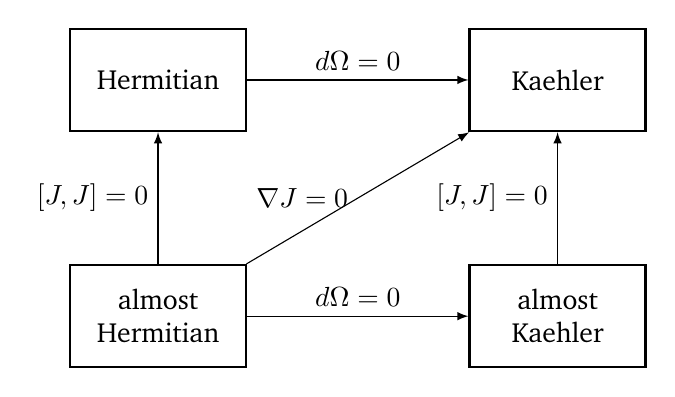
\begin{tikzpicture}  
\node[block] (a) {Hermitian};   
\node[block,right=80pt of a] (b) {Kaehler};  
 % the commands used for the different location of different blocks   
 \node[block] (c) at ([yshift=-3cm]$(a)!1.0!(a)$) {almost Hermitian};  
  \node[block] (d) at ([yshift=-3cm]$(b)!1.0!(b)$) {almost Kaehler};   
  \draw[line] (a)--node[above]{$d\Omega =0$} (b);  
  \draw[line] (d)-- node[left]{$[J,J]=0$} (b);  
  \draw[line] (c)-- node[left]{$[J,J]=0$} (a);   
  \draw[line] (c)-- node[above]{$d\Omega =0$}(d);
  \draw[line] (c)--node[left]{$\nabla J=0$}  (b);
\end{tikzpicture}  
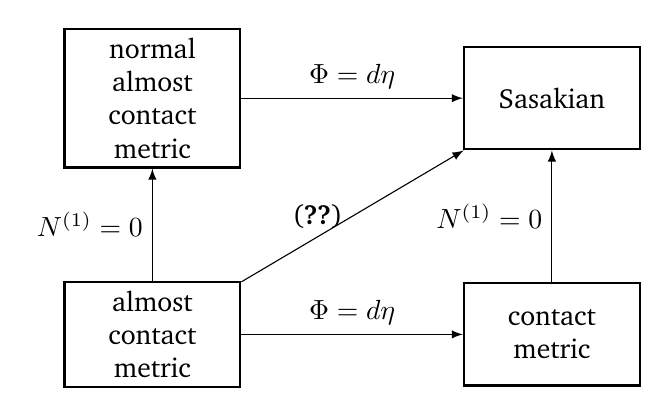
\begin{tikzpicture}  
\node[block] (a) {normal almost contact metric};   
\node[block,right=80pt of a] (b) {Sasakian};  
 % the commands used for the different location of different blocks   
 \node[block] (c) at ([yshift=-3cm]$(a)!1.0!(a)$) {almost contact metric};  
  \node[block] (d) at ([yshift=-3cm]$(b)!1.0!(b)$) { contact metric};   
  \draw[line] (a)--node[above]{$\Phi=d \eta$} (b);  
  \draw[line] (d)-- node[left]{$N^{(1)}=0$} (b);  
  \draw[line] (c)-- node[left]{$N^{(1)}=0$} (a);   
  \draw[line] (c)-- node[above]{$\Phi=d \eta$}(d);
  \draw[line] (c)--node[left]{$\eqref{eq28}$}  (b);
\end{tikzpicture}  





\subsection{More about Sasakian manifolds}

Recall that
    a \textbf{contact metric structure} on an odd-dimensional manifold $N^{2 n+1}$ is given by $(\varphi, \xi, \eta, g)$, where $\varphi$ is a tensor field of type $(1,1)$ on $N, \xi$ is a vector field, $\eta$ is an 1-form and $g$ is a Riemannian metric such that
    \begin{equation}\label{eq1}
        \varphi^2=-I+\eta \otimes \xi, \quad \eta(\xi)=1
    \end{equation}
and
\begin{equation}\label{eq2}
    g(\varphi X, \varphi Y)=g(X, Y)-\eta(X) \eta(Y), \quad g(X, \varphi Y)=d \eta(X, Y), \quad \forall X, Y \in C(T N) .
\end{equation}

\begin{remark} Recall that \cite{dragomir_differential_2006}, from $\eqref{eq1}$, one can deduce
    $$
\varphi \xi=0, \quad \eta \circ \varphi=0.
$$
\end{remark}

\begin{example}
    Strictly pseudoconvex CR manifolds are therefore contact Riemannian manifolds, in a natural way.
\end{example}
\begin{theorem}
   Let $\left(M, T_{1,0}(M), \theta\right)$ be a pseudo-Hermitian manifold. Then the Webster metric $g_\theta$ is Sasakian if and only if the Tanaka-Webster connection of $\left(M, T_{1,0}(M), \theta\right)$ has vanishing pseudo-Hermitian torsion, that is, $\tau=0$.
\end{theorem}

Recall that
    a contact metric manifold $(N, \varphi, \xi, \eta, g)$ is called \textbf{Sasakian} if it is normal, i.e.
$$
N_{\varphi}+2 d \eta \otimes \xi=0,
$$
where
\begin{equation}\label{eq:Jtorsion}
    N_{\varphi}(X, Y)=[\varphi X, \varphi Y]-\varphi[\varphi X, Y]-\varphi[X, \varphi Y]+\varphi^2[X, Y], \quad \forall X, Y \in C(T N),
\end{equation}
is the \textbf{Nijenhuis tensor} field of $\varphi$, or, equivalently, if
\begin{equation}
    \left(\nabla_X \varphi\right)(Y)=g(X, Y) \xi-\eta(Y) X, \quad \forall X, Y \in C(T N) .
\end{equation}

\begin{remark}
    We note that from the above formula it follows 
    \begin{equation}
        \nabla_X \xi=-\varphi X.
    \end{equation}
\end{remark}

\subsection{Connections and curvatures}

\begin{theorem}
 Let $\left(M, T_{1,0}(M), \theta\right)$ be a pseudo-Hermitian manifold and $g_\theta$ the Webster metric of $\left(M, T_{1,0}(M), \theta\right)$. Then there exists a unique linear connection $\nabla$ on $M$, called the \textbf{Tanaka-Webster} connection, such that:
 
(1) the Levi distribution $H(M)$ is parallel with respect to $\nabla$;

(2) $\nabla g_\theta=0, \nabla J=0, \nabla \theta=0$ (hence $\left.\nabla T=0\right)$;

(3) the torsion $T_{\nabla}$ of $\nabla$ satisfies $T_{\nabla}(X, Y)=-2 \Omega(X, Y) T$ and $T_{\nabla}(T, J X)=-J T_{\nabla}(T, X)$, for any $X, Y \in H(M)$.
\end{theorem}

We denote by $\nabla^\theta$ the Levi-Civita connection of $\left(M, g_\theta\right)$. One can see that the Levi-Civita connection $\nabla^\theta$ is related to the Tanaka-Webster connection $\nabla$ by
\begin{equation}\label{eq33}
    \nabla^\theta=\nabla+(\Omega-A) \otimes T+\tau \otimes \theta+2 \theta \odot J,
\end{equation}
where $2(\theta \odot J)(X, Y)=\theta(X) J Y+\theta(Y) J X$. Thus, we have $\nabla_X^\theta T=$ $\tau(X)+J X$. In particular, 
\begin{equation}
    \nabla_T^\theta T=0.
\end{equation}
If $X, Y \in H(M)$, then
\begin{equation}
    \nabla_X^\theta Y=\nabla_X Y+[\Omega(X, Y)-A(X, Y)] T .
\end{equation}
Since $\nabla^\theta-\nabla$ is a $(1,2)$ tensor field on $M$ and $\nabla_T^\theta T=\nabla_T T=0$, we can define a vector field $V$ on $M$ given by
\begin{equation}
    V=\operatorname{trace}_{g_\theta}\left(\nabla^\theta-\nabla\right)=\operatorname{trace}_{G_\theta}\left(\nabla^\theta-\nabla\right) .
\end{equation}
Actually we have 
\begin{equation}
    V=-\operatorname{trace}_{g_\theta}(\tau) T=0
\end{equation}







\begin{definition}
    Let $(N, \varphi, \xi, \eta, g)$ be a Sasakian manifold. The sectional curvature of a 2 -plane generated by $X$ and $\varphi X$, where $X$ is an unit vector orthogonal to $\xi$, is called the $\varphi$-\textbf{sectional curvature} determined by $X$. If the $\varphi$-sectional curvature is a constant $c$, then $(N, \varphi, \xi, \eta, g)$ is called a \textbf{Sasakian space form} and it is denoted by $N(c)$.
The curvature tensor field of a Sasakian space form $N(c)$ is given by
\begin{equation}
    \begin{aligned}
R(X, Y) Z= & \frac{c+3}{4}\{g(Z, Y) X-g(Z, X) Y\}+\frac{c-1}{4}\{\eta(Z) \eta(X) Y- \\
& -\eta(Z) \eta(Y) X+g(Z, X) \eta(Y) \xi-g(Z, Y) \eta(X) \xi+ \\
& +g(Z, \varphi Y) \varphi X-g(Z, \varphi X) \varphi Y+2 g(X, \varphi Y) \varphi Z\}
\end{aligned}
\end{equation}
\end{definition}

\begin{remark}[cf. \cite{chen_bochner-type_2012}]
    The $\varphi$-sectional curvature determines the curvature tensor $R$ completely.
\end{remark}

\begin{remark}
    A direct consequence of $\eqref{eq33}$ is that, for Sasakian manifolds, we have(substitute $\tau=0, A=0$ )
    \begin{equation}
        K(X, JX)=K^{\theta}(X,JX)+3, \forall X \in \mathcal{H}(M),
    \end{equation}
    and 
    \begin{equation}
        K(X, T)=K^{\theta}(X,T)-1=0, \forall X \in \mathcal{H}(M),
    \end{equation}
    where $K$ is sectional curvature wrt TW connection, while $K^{\theta}$ is the sectional curvature wrt LC connection.
\end{remark}

\begin{theorem}[cf. \cite{blair_riemannian_2010}]
     Let $M(c)$ be a complete, simply connected Sasakian manifold with constant $\phi$-sectional curvature $c$. Then $M(c)$ belongs one of the three families of examples listed below.
\end{theorem}

To begin, let $(\phi, \xi, \eta, g)$ be a contact metric structure and recall the notion of a $\mathcal{D}$-\textbf{homothetic deformation}:
\begin{equation}\label{eq6}
    \bar{\eta}=a \eta, \quad \bar{\xi}=\frac{1}{a} \xi, \quad \bar{\phi}=\phi, \quad \bar{g}=a g+a(a-1) \eta \otimes \eta,
\end{equation}
where $a$ is a positive constant. The deformed structure $(\bar{\phi}, \bar{\xi}, \bar{\eta}, \bar{g})$ is again a contact metric structure, and it enjoys many of the properties of the original structure. In particular, if $(\phi, \xi, \eta, g)$ is Sasakian, so is $(\bar{\phi}, \bar{\xi}, \bar{\eta}, \bar{g})$; if $M(c)$ is a Sasakian space form, then deforming the structure, we obtain the Sasakian space form $M(\bar{c})$ where $$\bar{c}=\frac{c+3}{a}-3$$ (see Tanno [1968], [1969] for details). We will show that there exist Sasakian space forms $M(c)$ for every value of $c$. 

\begin{remark}
    $\eqref{eq6}$ is natural from my point of view: we want to make a conformal transformation on $\mathcal{D}$ or ,more precisely, homothetic deformation,  so we hope when restricting to $\mathcal{D}$: $\bar{g}=ag$, so we may assume $\bar{g}=ag+b\eta\otimes \eta.$ But from the 2nd of $\eqref{eq2}$, we are suggested to let $\bar{\eta}=a\eta$ so $\bar{\xi}$ follows its step. Now put the above transformations to the 1st of $\eqref{eq2}$ (testing $\bar{\xi}$), we get $b=a^2-a$.
\end{remark}

\begin{example}[$\mathbb{S}^{2 n+1}, c>-3$]
    Let $\mathbb{S}^{2 n+1}=\left\{z \in \mathbb{C}^{n+1}:|z|=1\right\}$ be the unit $(2 n+1)$-dimensional Euclidean sphere. Consider the following structure tensor fields on $\mathbb{S}^{2 n+1}$ : the standard metric field $g_0$, the vector field $\xi_0(z)=-\mathcal{J} z, z \in \mathbb{S}^{2 n+1}$, where $\mathcal{J}$ is the usual almost complex structure on $\mathbb{C}^{n+1}$ defined by
$$
\mathcal{J} z=\left(-y^1, \ldots,-y^{n+1}, x^1, \ldots, x^{n+1}\right),
$$
for $z=\left(x^1, \ldots, x^{n+1}, y^1, \ldots, y^{n+1}\right)$, and $\varphi_0=s \circ \mathcal{J}$, where $s: T_z \mathbb{C}^{n+1} \rightarrow T_z \mathbb{S}^{2 n+1}$ denotes the orthogonal projection.  Then $g_0$ and $\xi_0$ detemine $\eta_0$ and $\varphi_0$ by 
$$
\eta_0=g_0(\xi_0,\cdot), \quad d\eta_0(X,Y)=2g( X,\varphi_0 Y).
$$
Equipped with these tensors, $\mathbb{S}^{2 n+1}$ becomes a Sasakian space form with the $\varphi_0$-sectional curvature equal to 1 , denoted by $\mathbb{S}^{2 n+1}(1)$. Now, consider the deformed structure on $\mathbb{S}^{2 n+1}$
$$
\eta=a \eta_0, \quad \xi=\frac{1}{a} \xi_0, \quad \varphi=\varphi_0, \quad g=a g_0+a(a-1) \eta_0 \otimes \eta_0
$$
where $a$ is a positive constant. The structure $(\varphi, \xi, \eta, g)$ is still a Sasakian structure and $\left(\mathbb{S}^{2 n+1}, \varphi, \xi, \eta, g\right)$ is a Sasakian space form with constant $\varphi$-sectional curvature $c=\frac{4}{a}-3$, $c>-3$, denoted by $\mathbb{S}^{2 n+1}(c)$.
\end{example}

\begin{example}[$\mathbb{R}^{2 n+1}, c=-3$]
    The Euclidean space $\mathbb{R}^{2 n+1}\left(x^1, \ldots, x^n, y^1, \ldots, y^n, z\right)$ is a Sasaki manifold with Sasaki structure $(\xi, \eta, \phi, g)$ as follows:
$$
\begin{gathered}
\xi=2 \frac{\partial}{\partial z}, \quad \eta=\frac{1}{2}\left(d z-\sum_{i=1}^n y^i d x^i\right), \quad g=\eta \otimes \eta+\frac{1}{4} \sum_{i=1}^n\left(\left(d x^i\right)^2+\left(d y^i\right)^2\right), \\
\phi\left(\frac{\partial}{\partial x^i}\right)=-\frac{\partial}{\partial y^i}, \quad \phi\left(\frac{\partial}{\partial y^i}\right)=\frac{\partial}{\partial x^i}+y^i \frac{\partial}{\partial z}, \quad \phi\left(\frac{\partial}{\partial z}\right)=0 .
\end{gathered}
$$
\end{example}

\begin{example}[$B^n \times \mathbb{R}, c<-3$]
    Let $B^n$ be a simply connected bounded domain in $\mathbb{C}^n$ and $(J, G)$ a Kähler structure with constant holomorphic sectional curvature $k<0$. For such a structure, the fundamental 2 -form $\Omega$ of the Kähler structure is exact and hence $\Omega=d \omega$ for some real analytic 1 -form $\omega$. Now on $B^n \times \mathbb{R}$ let $\pi$ denote the projection onto $B^n$ and $t$ the coordinate on $\mathbb{R}$. Then $B^n \times \mathbb{R}$ with $\eta=\pi^* \omega+d t$ and $g=\pi^* G+\eta \otimes \eta$ is a Sasakian manifold. Regarding $\eta$ as a connection form on $B^n \times \mathbb{R}$, let $\tilde{\pi} X$ denote the horizontal lift of a vector field $X$ on $B^n$. Also we denote by $\underline{K}$ the sectional curvature of $B^n$. Then by direct computation (see Ogiue [1965] or use the Riemannian submersion technique of O'Neill [1966]), we have $K(\tilde{\pi} X, \tilde{\pi} Y)=\underline{K}(X, Y)-3 \eta\left(\nabla_{\tilde{\pi} X} \tilde{\pi} Y\right)^2$ where $\{X, Y\}$ is an orthonormal pair on $B^n$. Now $g\left(\nabla_{\tilde{\pi} X} \tilde{\pi} Y, \xi\right)=-g\left(\tilde{\pi} Y, \nabla_{\tilde{\pi} X} \xi\right)=g(\tilde{\pi} Y, \phi \tilde{\pi} X)=$ $g(\tilde{\pi} Y, \tilde{\pi} J X)$. Therefore $B^n \times \mathbb{R}$ has constant $\phi$-sectional curvature $c=$ $k-3$
\end{example}

The following is a Sasakian analogue of Schur’s Theorem.
\begin{theorem}[cf. \cite{adachi_geometric_2010}]
     If the $\phi$-sectional curvature at each point of a Sasakian manifold $M$ of dimension $\geq 5$ does not depend on the choice of $\phi$-section at that point, then it is constant on $M$.
\end{theorem}

The following is the unique
existence theorem of Sasakian space forms.
\begin{theorem}
    For any two simply connected complete Sasakian manifolds of constant $\phi$-sectional curvature $c$, there exists an isomorphism between them which preserves their almost contact metric structures.
\end{theorem}



\chapter{CR Manifolds}
\textcolor{blue}{Note that the wedge $\wedge $  is taken by Alt convention, not Det convention as usual.}

\section{CR manifolds}
Let $M$ be a $m$-dimensional smooth manifold.  Let $n\in \nn$ be an integer s.t. $1\leq n \leq [m/2]$.  
\begin{definition}
    A complex subbundle $T_{1,0}(M)$ of the complexified tangent bundle $T(M) \otimes \mathbb{C}$, of complex rank $n$, is called \textbf{an almost complex CR structure} if 
    $$
T_{1,0}(M) \cap T_{0,1}(M)=(0).
$$ 
Here $ T_{0,1}(M)=\overline{T_{1,0}(M)}$. The integers $n$ and $k=m-2n$ are respectively the CR dimension and CR codimension of the almost CR structure and $(n,k)$ is its type.    
\end{definition}
\begin{remark}[cf. \cite{dragomirDifferentialGeometryAnalysis2006}]
An almost CR manifold of type $(n,0) $ is an almost complex manifold.  
\end{remark}
\begin{definition}
    An almost CR structure is \textbf{formally integrable} if
    $$
\left[\Gamma^{\infty}\left(U, T_{1,0}(M)\right), \Gamma^{\infty}\left(U, T_{1,0}(M)\right)\right] \subseteq \Gamma^{\infty}\left(U, T_{1,0}(M)\right).
$$
If this is the case, $T_{1,0}(M)$ is referred to as a\textbf{ CR structure} and $(M,T_{1,0}(M))$ is a \textbf{CR manifold. } 
\end{definition}
\begin{definition}
    A smooth map $f$ between two CR manifolds is called a \textbf{CR map} if   
    $$
\left(d_{x} f\right) T_{1,0}(M)_{x} \subseteq T_{1,0}(N)_{f(x)},
$$
where $df$ is the $\cc$-linear extension of the differential map.  
\end{definition}
\begin{remark}
    CR manifolds are the objects of a category whose arrows are smooth maps preserving CR structures. The  complex manifolds and holomorphic maps form a subcategory of the category of CR manifolds and CR maps.
\end{remark}

Let $\crm$ be a CR manifold of type $(n,k)$.
\begin{definition}
    The\textbf{ maximal complex} or \textbf{Levi distribution} of $\crm$ is  
    $$
H(M)=\operatorname{Re}\left\{T_{1,0}(M) \oplus T_{0,1}(M)\right\}.
$$
It carries the \textbf{complex structure} $J_{b}: H(M) \rightarrow H(M)$ given by
$$
J_{b}(V+\bar{V})=i(V-\bar{V}).
$$
Formally integrable condition is equivalent to
$$
\begin{gathered}
{\left[J_{b} X, Y\right]+\left[X, J_{b} Y\right] \in \Gamma^{\infty}(U, H(M)),} \\
{\left[J_{b} X, J_{b} Y\right]-[X, Y]=J_{b}\left\{\left[J_{b} X, Y\right]+\left[X, J_{b} Y\right]\right\}}
\end{gathered}
$$
CR map is equivalent to say
$$
\left(d_{x} f\right) H(M)_{x} \subseteq H(N)_{f(x)}
$$
and
$$
\left(d_{x} f\right) \circ J_{b, x}=J_{b, f(x)}^{N} \circ\left(d_{x} f\right).
$$
\end{definition}
  
\begin{definition}
   $ f : M \to N$ is a\textbf{ CR isomorphism} (or a CR equivalence) if $f$ is a smooth  diffeomorphism and a CR map.
\end{definition}

CR manifolds arise mainly as real submanifolds of complex manifolds. Let $V$ be a complex manifold, of complex dimension $N$ , and let $M \subset V$ be a real $m$-dimensional submanifold. Let us set
$$ T_{1,0}(M):=T^{1,0}(V) \cap T(M) \otimes \cc. $$
\begin{proposition}
    If $M$ is a real hypersurface $(m = 2N - 1)$, then$ T_{1,0}(M)$ is a CR structure of type $(N - 1, 1)$. 
\end{proposition}
In general the complex dimension of $T_{1,0}(M)$ defined above may not be constant. Nevertheless, if $ \dim _{\cc}T_{1,0}(M)\equiv n $, then $\crm$  is a CR manifold of type $(n,k)$.
\begin{definition}
    If the CR codimension of $\crm$ and the codimension of $M$ as a real submanifold of $V$ coincide, i.e., $k=2N-m$,  then $\crm$  is termed \textbf{ generic}.
\end{definition}
   

\subsection{Hypersurface type}
 Let 
$$ E_x=\{\omega \in T^{*}_x(M):H(M)_x \subset \ker (\omega )\} $$ 
Assume $M$ is orientable, then the bundle $E$ has a globally defined nowhere vanishing sections $\theta \in \Gamma (E)$.  
Given any \textbf{pseudo-Hermitian structure} $\theta$ on $M$ the \textbf{Levi form} $L_{\theta}$ is defined by
$$
\boxed{L_{\theta}(Z, \bar{W}):=-i(d \theta)(Z, \bar{W})=G_{\theta }(Z, \overline{W}).}
$$

\begin{remark}
The definition of Levi form of type $(n,k)$ could be possible, cf. \cite{dragomirDifferentialGeometryAnalysis2006}. 
\end{remark}

Define a bilinear form (also called \textbf{Levi form})
$$
\boxed{G_{\theta}(X, Y)=(d \theta)\left(X, J_{b} Y\right),}
$$
then
$$
\begin{aligned}
G_{\theta}\left(J_{b} X, J_{b} Y\right)-G_{\theta}(X, Y) & =-(d \theta)\left(J_{b} X, Y\right)-(d \theta)\left(X, J_{b} Y\right) \\
& =\frac{1}{2}\left\{\theta\left(\left[J_{b} X, Y\right]\right)+\theta\left(\left[X, J_{b} Y\right]\right)\right\} \\
& =\frac{1}{2} \theta\left(J_{b}\left\{[X, Y]-\left[J_{b} X, J_{b} Y\right]\right\}\right)=0.
\end{aligned}
$$
Define the $2$-form $\Omega$ by 
$$\boxed{\Omega(X,Y):=g_{\theta}(X,JY)=-d \theta (X,Y).} $$

\begin{definition}
    We say that $\left(M, T_{1,0}(M)\right)$ is \textbf{nondegenerate} if the Levi form $L_{\theta}$ is, the pair $(M, \theta)$ is referred to as a \textbf{pseudo-Hermitian manifold},
    and \textbf{strictly pseudoconvex} if $L_{\theta}$ is positive.
\end{definition}

\begin{remark}
Any two pseudo-Hermitian structure $\theta ,\hat{\theta }$ are related by 
\begin{equation}\label{eq:crtran}
    \hat{\theta }=\lambda \theta 
\end{equation}   
for some non-zero function $\lambda .$ Then Levi form changes according to 
$$ L_{\hat{\theta }}=\lambda L_{\theta }. $$ 
Hence non-degeneracy is a \textbf{CR-invariant} property, i.e., it is invariant under a transformation $\eqref{eq:crtran}.$ 
\end{remark}

\begin{definition}
    We say that a CR map $f: M \rightarrow N$ is a \textbf{pseudo-Hermitian map} if for some $c\in \mathbb{R}$,
    $$f^{*}\theta=c\theta. $$
    If $c=1$, then $f$ is referred to as an \textbf{isopseudo-Hermitian map}.
\end{definition}

\begin{definition}[Webster metric]
    $$
g_{\theta}(X, Y)=G_{\theta}(X, Y), \quad g_{\theta}(X, T)=0, \quad g_{\theta}(T, T)=1
$$
$$
\boxed{g_{\theta}=\pi_{H} G_{\theta}+\theta \otimes \theta.}
$$
\end{definition}
\begin{proposition}[Reeb vector field]
  There is a unique globally defined nowhere zero tangent vector field $T$ on $M$ such that
  $$ \theta (T)=1, \quad T \rfloor \, d \theta =0.
  $$
\end{proposition}



\subsubsection{CR geometry and contact Riemannian geometry}
Let $M$ be a $(2n+1)$-dimensional smooth manifold. Let $(\phi,\xi,\eta)$
be a synthetic object, consisting of a $(1, 1)$-tensor field $\phi: T (M) \to T (M)$, a tangent
vector field $\xi \in \mathcal{X}(M)$, and a differential $1$-form $\eta$ on $M$. Then $(\phi,\xi,\eta)$ is an \textbf{almost contact structure} if
$$
\phi^{2}=-I+\eta \otimes \xi, \quad \phi \xi=0, \quad \eta(\xi)=1, \quad \eta \circ \phi=0 .
$$
An almost contact structure $(\phi,\xi,\eta)$ is said to be \textbf{normal} if (recall $ \eqref{eq:Jtorsion} $)
$$
[\phi, \phi]+2(d \eta) \otimes \xi=0.
$$
A Riemannian metric $g$ on $M$ is said to be \textbf{compatible} with the almost contact structure $(\phi,\xi,\eta)$ if
$$
g(\phi X, \phi Y)=g(X, Y)-\eta(X) \eta(Y).
$$
A synthetic object $(\phi,\xi,\eta,g)$ consisting of an almost contact
structure $(\phi,\xi,\eta)$ and a compatible Riemannian metric $g$ is said to be an \textbf{almost contact metric structure}. 

Given an almost contact metric structure $(\phi,\xi,\eta,g)$ one defines
a $2$-form $\Omega$ by setting $$\Omega(X, Y ) = g(X, \phi Y ).$$  

$(\phi,\xi,\eta,g)$ is said to satisfy the \textbf{contact condition }if $\Omega = d\eta$, and if this is the case, $(\phi,\xi,\eta,g)$ is called a \textbf{contact metric structure }on $M$. 

A contact metric structure $(\phi,\xi,\eta,g)$ that is also normal is called a \textbf{Sasakian structure} (and $g$ is a \textbf{Sasakian metric}).

\begin{example}
    Strictly pseudoconvex CR manifolds are contact Riemannian manifolds, in a natural way.
    In fact,
    $$
\begin{aligned}
J_{b}^{2} & =-I+\theta \otimes T, \\
J_{b} T & =0, \quad \theta \circ J_{b}=0, \quad g_{\theta}(X, T)=\theta(X), \\
g_{\theta}\left(J_{b} X, J_{b} Y\right) & =g_{\theta}(X, Y)-\theta(X) \theta(Y),
\end{aligned}
$$
and
$$\Omega=-d\theta.$$
\end{example}

\begin{theorem}[\cite{dragomirDifferentialGeometryAnalysis2006}]
    Let $(M, T_{1,0} (M), \theta)$ be a pseudo-Hermitian manifold. Then the Webster metric $g_{\theta}$ is Sasakian if and only if the Tanaka-Webster connection $\nabla$ has vanishing \textbf{pseudo-Hermitian torsion}, that is, $\tau=0.$ 
\end{theorem}
\begin{remark}
    The pseudo-Hermitian torsion of $\nabla $,  $\tau$ is defined by 
    $$\boxed{\tau(X)=T_{\nabla}(T,X).}$$ 
    $T_{\nabla}$ is torsion tensor of the Tanaka–Webster connection.
\end{remark}

\begin{theorem}[Tanaka-Webster connection on pseudo-Hermitian manifold]
    There exists a connection $\nabla$ with the following properties:\\
    1. $H(M)$ is parallel w.r.t. $\nabla$;\\
    2. $\nabla g_{\theta}=0,\nabla J=0, \nabla \theta =0,\nabla T=0.$\\
    3. $T_{\nabla}(X,Y)=-2\Omega(X,Y)T, T_{\nabla}(T,JX)=-JT_{\nabla}(T,X)$.
\end{theorem}

\begin{remark}
    We say $T_{\nabla}$ is \textbf{pure} if
    \begin{align}
    T_{\nabla}(Z, W) & =0 \\
    T_{\nabla}(Z, \bar{W}) & =2 i L_{\theta}(Z, \bar{W}) T \label{eq:pure2}\\
    \tau \circ J+J \circ \tau & =0
    \end{align}
\end{remark}

\begin{theorem}[Tanaka-Webster connection]
    Let $(M, T_{1,0}(M),\theta) $ be a nondegenerate CR manifold. Then there is a unique linear connection $ \nabla  $ on $M$ satisfying the following axioms:
    \begin{enumerate}[(i)]
        \item $H(M)$ is parallel w.r.t. $\nabla$.
        \item $ \nabla J =0,\quad \nabla g_{\theta }=0. $
        \item $ T_{\nabla } $ is pure.
    \end{enumerate}
\end{theorem}
\begin{proof}
    Let $ \pi _{\pm}: T_{\cc}M \to T_{1,0}(M)~ (T_{0,1}(M)) $ be the natural projections. Then $ \pi _{-}Z=\overline{\pi _{+} \bar{Z} }$. Note also that 
    $$ T_{\cc}M=T_{1,0}(M) \oplus T_{1,0}(M) \oplus \cc T.$$

    \textbf{Uniqueness}: From $ \eqref{eq:pure2} $, 
    $$ [\bar{Y}, Z]=\nabla_{\bar{Y}} Z-\nabla_Z \bar{Y}+2 i L_\theta(Z, \bar{Y}) T, \quad \forall Y,Z \in T_{1,0}(M) .$$

\end{proof}

\begin{proposition}\label{pr:connection}
    The following formulas hold:
   $$ \boxed{T_{\nabla }=2(\theta  \wedge \tau -\Omega \otimes  T) }$$ 
   $$ \boxed{\nabla ^{\theta }=\nabla +(\Omega -A)T+\tau  \otimes \theta +2 \theta \odot  J }$$
   $$ \trace_{g_{\theta }}(\nabla ^{\theta }-\nabla )=\trace_{G_{\theta }}(\nabla ^{\theta }-\nabla )=0. $$
\end{proposition}


\begin{theorem}
  The curvatures of  TW connection and LC connection  are related by 
  $$ \begin{aligned}
    R^\theta(X, Y) Z=R(X, Y) & Z+(L X \wedge L Y) Z-2 \Omega(X, Y) J Z \\
    & -g_\theta(S(X, Y), Z) T+\theta(Z) S(X, Y) \\
    & -2 g_\theta((\theta \wedge \mathcal{O})(X, Y), Z) T+2 \theta(Z)(\theta \wedge \mathcal{O})(X, Y),
    \end{aligned} $$
    for any $X,Y,Z \in TM$. 
    where 
    $$ S(X,Y)=(\nabla _{X}\tau )Y-(\nabla _{Y}\tau )X ,$$
    $$ \mathcal{O}=\tau ^2+2J \tau -I ,\quad L=\tau +J.$$
\end{theorem}
\begin{remark}
   Note that 
   $$ J^2Y=-Y+\theta (Y)T, \quad \forall Y \in TM. $$ 
\end{remark}

\begin{theorem}[Structure equations for TW connection]
    \begin{equation}
    \begin{aligned}
d\theta & =2\sqrt{-1}h_{\alpha\bar{\beta}}\theta^{\alpha}\wedge\theta^{\bar\beta},  \\
d\theta^{\alpha}& =\theta^\beta\wedge\omega_\beta^\alpha+\theta\wedge\tau^\alpha, & dh_{\alpha\bar{\beta}}=\omega_{\alpha}^{\gamma}h_{\gamma\bar{\beta}}+h_{\alpha\bar{\gamma}}\omega_{\bar{\beta}}^{\bar{\gamma}},  \\
d\omega_\beta^{\alpha}& =-\omega_\gamma^\alpha\wedge\omega_\beta^\gamma+\Pi_\beta^\alpha, 
\end{aligned}
\end{equation}
where
\begin{equation}
\begin{aligned}
\Pi_\beta^\alpha&=R_{\beta\gamma\bar\delta}^\alpha\theta^\gamma\wedge\theta^{\bar\delta}+W_{\beta\gamma}^\alpha\theta^\gamma\wedge\theta-W_{\beta\bar\gamma}^\alpha\theta^{\bar\gamma}\wedge\theta\\&
+2\sqrt{-1}\theta_\beta\wedge\tau^\alpha-2\sqrt{-1}\tau_\beta\wedge\theta^\alpha,
\end{aligned}
\end{equation}
and
\begin{equation}
    W_{\alpha \bar{\gamma}}^{\beta}=h^{\bar{\delta} \beta} A_{\bar{\gamma} \bar{\delta}, \alpha}, \quad W_{\alpha \gamma}^{\beta}=h^{\bar{\delta} \beta} A_{\alpha \gamma, \bar{\delta}}, \quad \tau_{\alpha}=h_{\alpha \bar{\beta}} \tau^{\bar{\beta}}, \quad \theta_{\alpha}=h_{\alpha \bar{\beta}} \theta^{\bar{\beta}}.
\end{equation}
\end{theorem}
\begin{remark}
    \begin{equation}
d\theta^{\bar\alpha}=\theta^{\bar\beta}\wedge\omega_{\bar\beta}^{\bar\alpha}+\theta\wedge\tau^{\bar\alpha}
    \end{equation}
\end{remark}

\section{Divergence formulas}
\begin{definition}
    Define the divergence of a vector $X \in TM$  by 
    $$ \di (X) \Psi  = \mathcal{L}_{X} \Psi ,$$
    where $\Psi $ is a volume form. 
\end{definition}
\begin{remark}
   We can take 
   $$ \Psi = \theta \wedge (d \theta )^n .$$ 
\end{remark}
\begin{remark}
    By 3rd relation of Proposition \ref{pr:connection}, 
   $$ \di (X)= \trace_{g_{\theta }}\{Y \in TM \to \nabla _{Y}X\} .$$ 
   Note that 
   $$ \begin{aligned}
   g_{\theta }(\nabla ^{\theta }_{e_{A}}X,e_{A})= g_{\theta }(\nabla ^{\theta }_{T_{\alpha }}X,T_{\bar \alpha })+g_{\theta }(\nabla ^{\theta }_{T_{\bar\alpha }}X,T_{ \alpha })+g_{\theta }(\nabla ^{\theta }_{T}X,T),
   \end{aligned}  $$
   assuming $\{T_{\alpha }\} $ is orthonormal and $T_{\alpha }=\frac{1}{\sqrt{2}}(e_{\alpha }-iJ e_{\alpha }) $.  
\end{remark}
\begin{exercise}
    For any complex vector $Z \in T_{\cc}(M)$, 
    $$ \overline{\di (Z)}=\di (\bar{Z}) .$$
\end{exercise}
\begin{definition}
    Define  the divergence of a 1-form $\sigma $ by 
    $$ \di (\sigma )=\di (X_{\sigma }), $$ 
    where $X_{\sigma }$ is the dual vector of $\sigma $ w.r.t. $g_{\theta }$, i.e., $g_{\theta }(X_{\sigma },Y)=\sigma (Y), \forall  Y \in TM $.    
\end{definition}
\begin{exercise}
$$ \di (Z)=T_{\alpha }(Z^{\alpha })+Z^{\beta } \omega _{\beta }^{\alpha }(T_{\alpha }), \quad \forall  Z=Z^{\alpha }T_{\alpha }\in T_{1,0}(M).$$
$$ \di (\sigma )=\sigma _{\alpha ,\bar{\beta }}h^{\alpha \bar{\beta }}. $$
\end{exercise}

\begin{definition}
    Sublaplacian for functions is defined by 
    $$ \Delta _b(u):=-\di(\nabla^{\mathcal{H}} u)=-(u_{\alpha \bar{\beta }}h^{\alpha \bar{\beta }}+u_{\bar{\alpha }\beta }h^{\bar{\alpha }\beta }) ,$$
    where $\nabla ^{\mathcal{H}}u$ is the horizontal component of the gradient $\nabla u$.  
\end{definition}
\begin{exercise}
    The usual Laplacian is given by 
    $$ \Delta  u= -(u_{\alpha \bar{\beta }}h^{\alpha \bar{\beta }}+u_{\bar{\alpha }\beta }h^{\bar{\alpha }\beta }+u_{00}). $$
\end{exercise}










\chapter{Geometry of CR-Submanifolds}

\section{CR-submanifolds and CR-structures}
Let $N$ be a $n$-dimensional \textit{almost Hermitian manifold} with almost complex structure $J$ and with Hermitian metric $g$. Let $M$ be a \textit{real} $m$-dimensional Riemannian manifold isometrically immersed in $N$.

\begin{definition}
    The differential geometry of $M$ depends on the behaviour of the tangent bundle of $M$ relative to the action of the almost complex structure $J$. Thus $M$ is called a \textbf{\textit{complex} (holomorphic)} submanifold if $T_xM$ is invariant by $J$, i.e., we have
$$
J(T_xM) = T_xM, \quad \text{for each } x \in M.
$$
Also, we say that $M$ is a \textbf{\textit{totally real} (anti-invariant)} submanifold of $N$ if we have
$$
J(T_xM) \subseteq T_xM^{\perp}, \quad \text{for each } x \in M.
$$
These two classes of submanifolds have been extensively investigated in the last decade from different viewpoints.
\end{definition}

\begin{definition}
    In 1978 ``we" (refer to the author of \cite{bejancuGeometryCRSubmanifolds1986}) initiated a study of the differential geometry of a new class of submanifolds situated between the above two classes, called CR-submanifolds. More precisely, $M$ is said to be a \textbf{CR-submanifold} of $N$ if there exists a differentiable distribution
\[
D: x \mapsto D_x \subseteq T_xM,
\]
on $M$ satisfying the following conditions:
\begin{enumerate}
    \item[(i)] $D$ is holomorphic, i.e., $J(D_x) = D_x$ for each $x \in M$,
    \item[(ii)] the complementary orthogonal distribution
    \[
    D^{\perp}: x \mapsto D^{\perp}_x \subseteq T_xM^{\perp},
    \]
    is anti-invariant, i.e., $J(D^{\perp}_x) \subseteq (T_xM)^{\perp}$ for each $x \in M$.
\end{enumerate}
We denote by $p$ the complex dimension of the distribution.
D and by $q$ the real dimension of the distribution $D^\perp$. Then for $q = 0$ (resp. $p = 0$) a CR-submanifold becomes a \textbf{complex submanifold (resp. totally real submanifold)}. If $q = \dim T_xM^\perp$ the CR-submanifold is called an \textbf{anti-holomorphic submanifold}. A \textbf{proper CR-submanifold} is a CR-submanifold which is neither a complex submanifold nor a totally real submanifold.
\end{definition}

\begin{example}
    Each real hypersurface $M$ of $N$ (with $n \geq 2$) is a proper CR-submanifold. In fact we define
\[
D_x^\perp : x \mapsto D_x^\perp = J(T_xM^\perp)
\]
and take $D$ as the complementary orthogonal distribution to $D^\perp$ in $TM$. Thus $M$ is endowed with a pair of distributions $(D, D^\perp)$ satisfying the conditions of the definition of a CR-submanifold. Moreover, we have $\dim _{\mathbb{R}} D_x^\perp = 1$ and $\dim_{\mathbb{C}} D_x = n - 1$.

Hence, $M$ is a proper CR-submanifold.
\end{example}


\begin{remark}
    It is easily seen that on a CR-submanifold the 
distribution \( D \) (resp. \( D^{\perp} \)) is the maximal distribution 
invariant by \( J \) (resp. anti-invariant by \( J \)), i.e., if \( D' \) 
(resp. \( D'' \)) is an invariant (resp. anti-invariant) distribution on \( M \), 
then we have \( D'_{x} \subseteq D_{x} \) (resp. \( D''_{x} \subseteq D_{x} \)), for each \( x \in M \).
\end{remark}

\begin{definition}
    Now let \( M \) be an arbitrary Riemannian manifold isometrically immersed in an almost Hermitian manifold \( N \). 
For each vector field \( X \) tangent to \( M \) we put
\begin{equation}
    JX = \phi X + \omega X,
\end{equation}
where \( \phi X \) and \( \omega X \) are respectively the tangent part and the normal part of \( JX \). Also, for each vector field \( V \) normal to \( M \) we put
\begin{equation}
    JV = BV + CV,
\end{equation}
where \( BV \) and \( CV \) are respectively the tangent part and the normal part of \( JV \).
\end{definition}


\begin{theorem}
     The submanifold \( M \) of \( N \) is a CR-submanifold if and only if we have
\[
\text{rank}(\phi) = \text{constant}, \omega\phi = 0.
\]
or, if and only if
\[
\text{rank}(B) = \text{constant}, \phi B = 0.
\]
\end{theorem}
\begin{remark}
Note that 
\begin{equation}
    \begin{aligned}
        &\phi X=JPX\\
        &\omega X=JQX
    \end{aligned}
\end{equation}
    for any $X\in TM$, $P, Q$ is the projection to $D, D^{\perp}$ respectively.

    Also, 
\begin{equation}
    \begin{aligned}
        &D=Im (\phi)=ker (\omega)\\
        &D^{\perp}=Im (B)=ker (\phi).
    \end{aligned}
\end{equation}
\end{remark}

\begin{remark}
     Now, suppose \( M \) is a CR-submanifold of the almost Hermitian manifold \( N \). 
    \begin{equation}
        \begin{aligned}
            \phi^2 = -P\\
            \phi^3 + \phi = 0\\
            C^3 + C = 0.
        \end{aligned}
    \end{equation}
\end{remark}


\begin{proposition}
    On each CR-submanifold \( M \) the vector bundle 
morphisms \( \phi \) and \( C \) define \( f \)-structures on \( TM \) and \( T^{\perp}M \) 
respectively.
\end{proposition}

\begin{theorem}[Blair-Chen]
    A CR-submanifold of a \textbf{Hermitian} manifold is a CR-manifold.
\end{theorem}

\section{f-structure}

Let \( M_n \) be an \( n \)-dimensional differentiable manifold of class \( C^{\infty} \) and 
let there be given a tensor field \( f \neq 0 \) of type \( (1,1) \) and of class \( C^{\infty} \) such that
\begin{equation}
f^3 + f = 0.
\label{eq:f_cubed_plus_f}
\end{equation}

\begin{theorem}[\cite{YANO1982251}]
    For a tensor field \( f \neq 0 \) satisfying \eqref{eq:f_cubed_plus_f}, the operators
\begin{equation}
l = -f^2, \quad m = f^2 + 1,
\label{eq:operators_l_m}
\end{equation}

\( 1 \) denoting the identity operator, applied to the tangent space at a point of the manifold are complementary projection operators.

Moreover,
\begin{equation}
fl = lf = f,
\label{eq:fl_lf_f}
\end{equation}
\begin{equation}
fm = mf = 0, lm=ml=0,
\label{eq:fm_mf}
\end{equation}
\begin{equation}
f^2 l = -l,
\label{eq:f2l}
\end{equation}
\begin{equation}
f^3 m = 0,
\label{eq:f3m}
\end{equation}
that is, \( f \) acts on \( L \) as an almost complex structure operator and on \( M \) as null operator.
\end{theorem}

\begin{remark}
    Thus if there is given a tensor field \( f \neq 0 \) satisfying $\eqref{eq:f_cubed_plus_f}$, then there exist 
complementary distributions \( L \) and \( M \) corresponding to the projection operators 
\( l \) and \( m \) respectively. 

Moreover, one can show that if the rank of \( f \) is constant and is equal to \( r \), 
then the dimensions of \( L \) and \( M \) are \( r \) and \( n-r \) respectively. We call such a structure 
an \( f \)-structure of rank \( r \).
\end{remark}

Let me mention that
\begin{theorem}[\cite{YANO1982251}]
     A necessary and sufficient condition for an \( n \)-dimensional 
manifold to admit a tensor field \( f \neq 0 \) of type \( (1,1) \) and of rank \( r \) such 
that \( f^3 + f = 0 \) is that \( r \) is even: \( r = 2m \) and the group of tangent bundle 
of the manifold be reduced to the group \( U(m) \times O(n-2m) \).
\end{theorem}


\section{Integrability of Distributions on a CR-Submanifold}
First of all, we have 
\begin{equation}
    [\phi, \phi](X, Y) = [\phi X, \phi Y] + \phi^2[X, Y] - \phi([\phi X, Y]) - \phi([X, \phi Y]).
\end{equation}
and
\begin{equation}
    [J, J](X, Y) = [\phi, \phi](X, Y) - \Omega([\phi X, Y] + [X, \phi Y]).
\end{equation}

\begin{theorem}[Bejancu]
Let \( M \) be a CR-submanifold of an 
almost Hermitian manifold \( N \). Then the distribution \( D \) is 
integrable if and only if
\begin{equation}
[J, J](X, Y)^{\perp} = 0
\end{equation}
and
\begin{equation}
Q(\phi, \phi)(X, Y) = 0, \text{ for any } X, Y \in \Gamma(D).
\end{equation}
\end{theorem}

\begin{corollary}
    Let $M$ be a CR-submanifold of a \textbf{Hermitian} manifold $N$. The distribution $D$ is integrable if and only if the Nijenhuis tensor of $\phi$ vanishes identically on $D$.
\end{corollary}

\begin{theorem}
    Let $M$ be a CR-submanifold of an almost Hermitian manifold $N$. The distribution $D$ is integrable if and only if the Nijenhuis tensor of $\phi$ vanishes identically on $D^{\perp}$.
\end{theorem}

\section{CR-submanifold of a nearly Kaehlerian manifold}
....

\section{\texorpdfstring{$\phi$}{phi}-Connections on a CR-Submanifold and CR-Products of Almost Hermitian Manifolds} 

\begin{definition}
    A linear connection $\nabla$ on $M$ is called a \textbf{$\phi$-connection} if $\phi$ is covariantly constant with respect to this connection, that is, we have
    \begin{equation}
        \nabla_X \phi =0, \forall X\in TM
    \end{equation}
\end{definition}

\begin{theorem}
    Both distributions $D$ and $D^{\perp}$ on a CR submanifold of an almost Hermitian manifold are parallel with respect to any $\phi$-connection.
\end{theorem}

\begin{definition}
    We say that a CR-submanifold \( M \) of an almost Hermitian manifold \( N \) 
is a \textbf{CR-product} if both distributions \( D \) and \( D^{\perp} \) are integrable 
and \( M \) is locally a Riemannian product \( M_1 \times M_2 \), where \( M_1 \) 
is a leaf of \( D \) and \( M_2 \) is a leaf of \( D^{\perp} \). 
A CR-product with \( D \neq \{0\} \) and \( D^{\perp} \neq \{0\} \) is called a 
\textbf{proper CR-product.}
\end{definition}

\begin{example}[An counterexample]
    There exist no proper CR submanifolds of $S^6$ with both distributions $D$ and $D^{\perp}$ parallel with respect to Levi-Civita connection. However, Sekigawa constructed  an example of a 3-dimensional proper CR-submanifold such that both distributions $D$ and $D^{\perp}$ are integrable.
\end{example}

\begin{theorem}
    Let \( M \) be a CR-submanifold of an 
almost Hermitian manifold \( N \). If the Levi-Civita connection 
on \( M \) is a \( \phi \)-connection, then \( M \) is a CR-product.
\end{theorem}
Recall that
\begin{theorem}
    Both distributions $D$ and $D^{\perp}$ are parallel with respect to Levi-Civita connection  if and only if they are integrable and their leaves are totally geodesic in $N$.
\end{theorem}

\section{CR-submanifolds of Kaehlerian manifolds}

\begin{theorem}
  Let \( M \) be a CR-submanifold of a K\"ahlerian manifold \( N \). Then we have
\begin{enumerate}
    \item[(i)] the distribution \( D^{\perp} \) is integrable,
    \item[(ii)] the distribution \( D \) is integrable if and only if the second fundamental form of \( M \) satisfies
    \[
    h(X, JY) = h(Y, JX), \text{ for any } X, Y \in \Gamma(D).
    \]
\end{enumerate}
\end{theorem}
\begin{remark}
    Blair and Chen have constructed  an example of a CR-submanifold of a Hermitian manifold for which $D^{\perp}$ is not integrable.
\end{remark}








 \bibliographystyle{plain}
 \bibliography{reference}
\end{document}
